\documentclass{article}

\usepackage[final]{neurips_2022}

\usepackage[utf8]{inputenc} % allow utf-8 input
\usepackage[T1]{fontenc}    % use 8-bit T1 fonts
\usepackage{hyperref}       % hyperlinks
\usepackage{url}            % simple URL typesetting
\usepackage{booktabs}       % professional-quality tables
\usepackage{amsfonts}       % blackboard math symbols
\usepackage{nicefrac}       % compact symbols for 1/2, etc.
\usepackage{microtype}      % microtypography
\usepackage{xcolor}         % colors
\usepackage{listings}
\usepackage{amsmath}
\usepackage{algorithm}
\usepackage{algpseudocode}
\usepackage{graphicx}
\graphicspath{ {./images/} }

\title{SafeRL}


\author{%
  Roopak Srinivasan \\
  (rs2386)\\
  % examples of more authors
  \And
  Yogesh Eshwar Patil \\
  (yp445) \\
  % \And
  % Name \\
  % (net-id) \\
}


\begin{document}


\maketitle


\section{Introduction}
Constrained Reinforcement Learning (RL) is a subfield of RL that focuses on learning policies that satisfy constraints while maximizing the reward. In many real-world applications, it is important to ensure that the agent does not violate certain constraints. One such important constraint is safety, where the agent must avoid unsafe actions that could lead to catastrophic failures.

In this project, we look at a Lunar Lander agent from Gymnasium environment \cite{lunar_lander_gym} that must land safely on the moon without crashing. We train two policies, base and safe models, using Proximal Policy Optimization (PPO) \cite{schulman2017proximal}. The base model is trained without any constraints, while the safe model is trained with constraints that enforce the agent to land within a certain parabolic curve trajectory. We evaluate the performance of both models in a new unknown world environment with high wind speeds and compare the performance of the base and safe models against the expert model of the unknown world environment. We analyze the trajectories of the Lunar Lander to understand how the policies differ in terms of safety.

\subsection{Lunar Lander Environment}
The Lunar Lander environment is a two-dimensional spacecraft that must land on the moon's surface within a certain distance of the landing pad. The agent must control the Lunar Lander's engines to adjust its position and velocity to land safely. The agent receives a reward based on its landing performance, with higher rewards for safer landings.

The environment 
\begin{figure}[h]
  \centering
  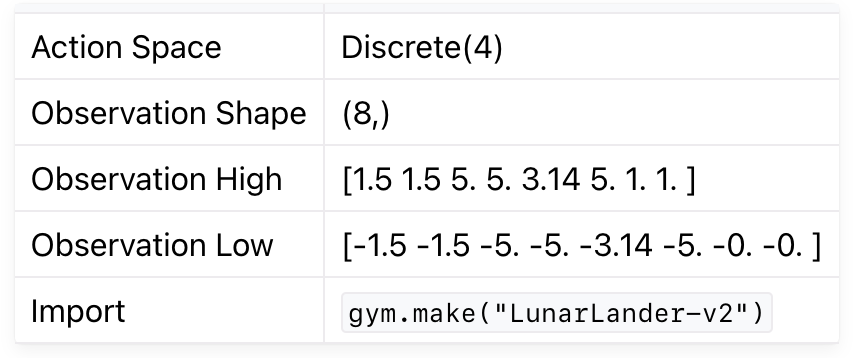
\includegraphics[width=0.5\textwidth]{lunar_lander_table.png}
  \caption{Lunar Lander Environment}
  \label{fig:environment_table}
\end{figure}

\section{Problem}
The problem we are trying to solve is to train a policy that can land the Lunar Lander safely on the moon without crashing. The Lunar Lander is a two-dimensional spacecraft that must land on the moon's surface within a certain distance of the landing pad. The goal is to maximize the reward while satisfying the constraints. 

\subsection{The Unknown World Environment}
The unknown world environment is a new environment  

\section{Approach}
\subsection{Defining the Environments}
We first define three environments: base, safe, and unknown world. The base environment is the standard Lunar Lander environment where the agent must land the Lunar Lander without any constraints. The safe environment is the Lunar Lander environment with constraints that enforce the agent to land within a certain parabolic curve trajectory. The unknown world environment is a new environment with high wind speeds that the agent has not seen during training.



\subsection{Training the Policies}

\begin{algorithm}
  \caption{Step Function for Lunar Lander Environment}
  \begin{algorithmic}[1]
  \Procedure{Step}{$action$}
      \State $observation, reward, done, \_, info \gets env.step(action)$
      \State $x, y \gets observation[0], observation[1]$
      \State $path.append((x, y))$
      \State $y_{desired} \gets a \cdot x^2 + b \cdot x + c$
      \If{$y < y_{desired}$}
          \State $deviation \gets y_{desired} - y$
          \State $penalty \gets -\sqrt{deviation} \cdot altitude\_scaling\_factor$
          \State $shaped\_reward \gets \max(max\_penalty, penalty)$
          \State $reward \gets reward + shaped\_reward$
          \If{$action \in \{1, 2, 3\}$}
              \State $reward \gets reward + reduced\_engine\_penalty + 0.3$
          \EndIf
      \EndIf
      \If{$done$}
          \State $info['safety'] \gets score\_landing\_path(x, y)$
      \EndIf
      \If{$done$ and $debug$}
          \State $SafePara.plot\_landing\_path(path, curving, x, y, info['safety'])$
      \EndIf
      \State \Return $observation, reward, done, \_, info$
  \EndProcedure
  \end{algorithmic}
  \end{algorithm}

\section{Results}

\bibliography{references}{}
\bibliographystyle{plain}

% \section*{References}

% Here are some examples (but feel free to use bib file if you want to)
% {
% \small

% [1] Alexander, J.A.\ \& Mozer, M.C.\ (1995) Template-based algorithms for
% connectionist rule extraction. In G.\ Tesauro, D.S.\ Touretzky and T.K.\ Leen
% (eds.), {\it Advances in Neural Information Processing Systems 7},
% pp.\ 609--616. Cambridge, MA: MIT Press.


% [2] Bower, J.M.\ \& Beeman, D.\ (1995) {\it The Book of GENESIS: Exploring
%   Realistic Neural Models with the GEneral NEural SImulation System.}  New York:
% TELOS/Springer--Verlag.


% [3] Hasselmo, M.E., Schnell, E.\ \& Barkai, E.\ (1995) Dynamics of learning and
% recall at excitatory recurrent synapses and cholinergic modulation in rat
% hippocampal region CA3. {\it Journal of Neuroscience} {\bf 15}(7):5249-5262.
% }


\end{document}